\chapter{FlexTouch Sensing Capability Evaluation}
In this section, we evaluate the sensing range of \textit{FlexTouch} considering the effects of several factors including fabrication materials, the signal strip's dimension, sensing hardware and the configuration of the grounding strip.

\section{Evaluating Sensing Range with Variable Fabrication Material, Hardware, and the Local Ground}

Fig ~\ref{fig:experiment} illustrates our hardware setup for this study. Two strips are coming out from the phone. The signal strip is directly attached to the phone touch surface by a plastic clamp, while the grounding strip is connected to the back plate of the phone. In this study, we only look at the difference between using and not using the grounding strip. We discuss other variables pertaining to the  grounding strip in a more thorough study in later parts of this section. 

\begin{figure}[ht]
	\centering
	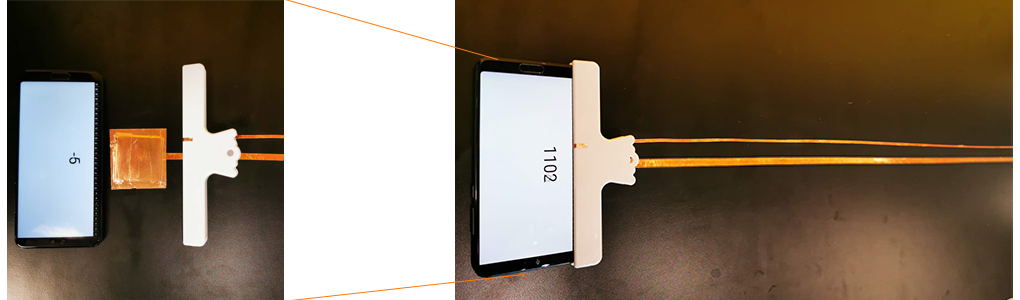
\includegraphics[width=0.95\columnwidth]{figures/evaluation_env.png}
	\setlength{\belowcaptionskip}{-6pt}
    \caption{Experiment setup to evaluate the touch sensing coverage range.}
    \label{fig:experiment}
\end{figure}
	
To evaluate the effect of different materials, We fabricated four different 5-meter long signal strips using materials including copper foil tape (CFT), ITO PET film (IPF), carbon paint (CP), and silver nanoparticle ink (SNI) with a fixed width of $1.5mm$. We set the grounding strip (5-meter long, $6mm$-wide copper foil tape) $2 cm$ away from the signal strip in this study. We recruited four participants for this experiment with an average age of 26.5 ($SD = 2.5$). The study lasted for 2 hours in total and we compensated each participant with a \$50 dollar gift card.

1) We attached the signal strip to the central position of the 8th sensing node on the touchscreen's left edge at the beginning of each session. In each session, we randomly selected two participants to perform a one-second finger touch on the far end of the signal strip five times followed by a one-second finger touch on the far end of both the signal and the grounding strips (also five times). Then we attached the signal strip to the 18th sensing node and repeat above procedure. 

2) We switched the phone hardware and repeated step 1).

3) We cut both signal and grounding strips to the next neighboring length following the order of 5m, 4m, 3m, 2.5m, 2m, 1.5m, 1m, 0.5m, 0.25m and 0.1m in sequence and repeated steps 1) and 2).

4) After completing the test on one material, we replaced it with another signal strip made of different material and repeated the experiment. Participants took a two-minute break between material switches.

\begin{figure}[ht]
	\centering
	  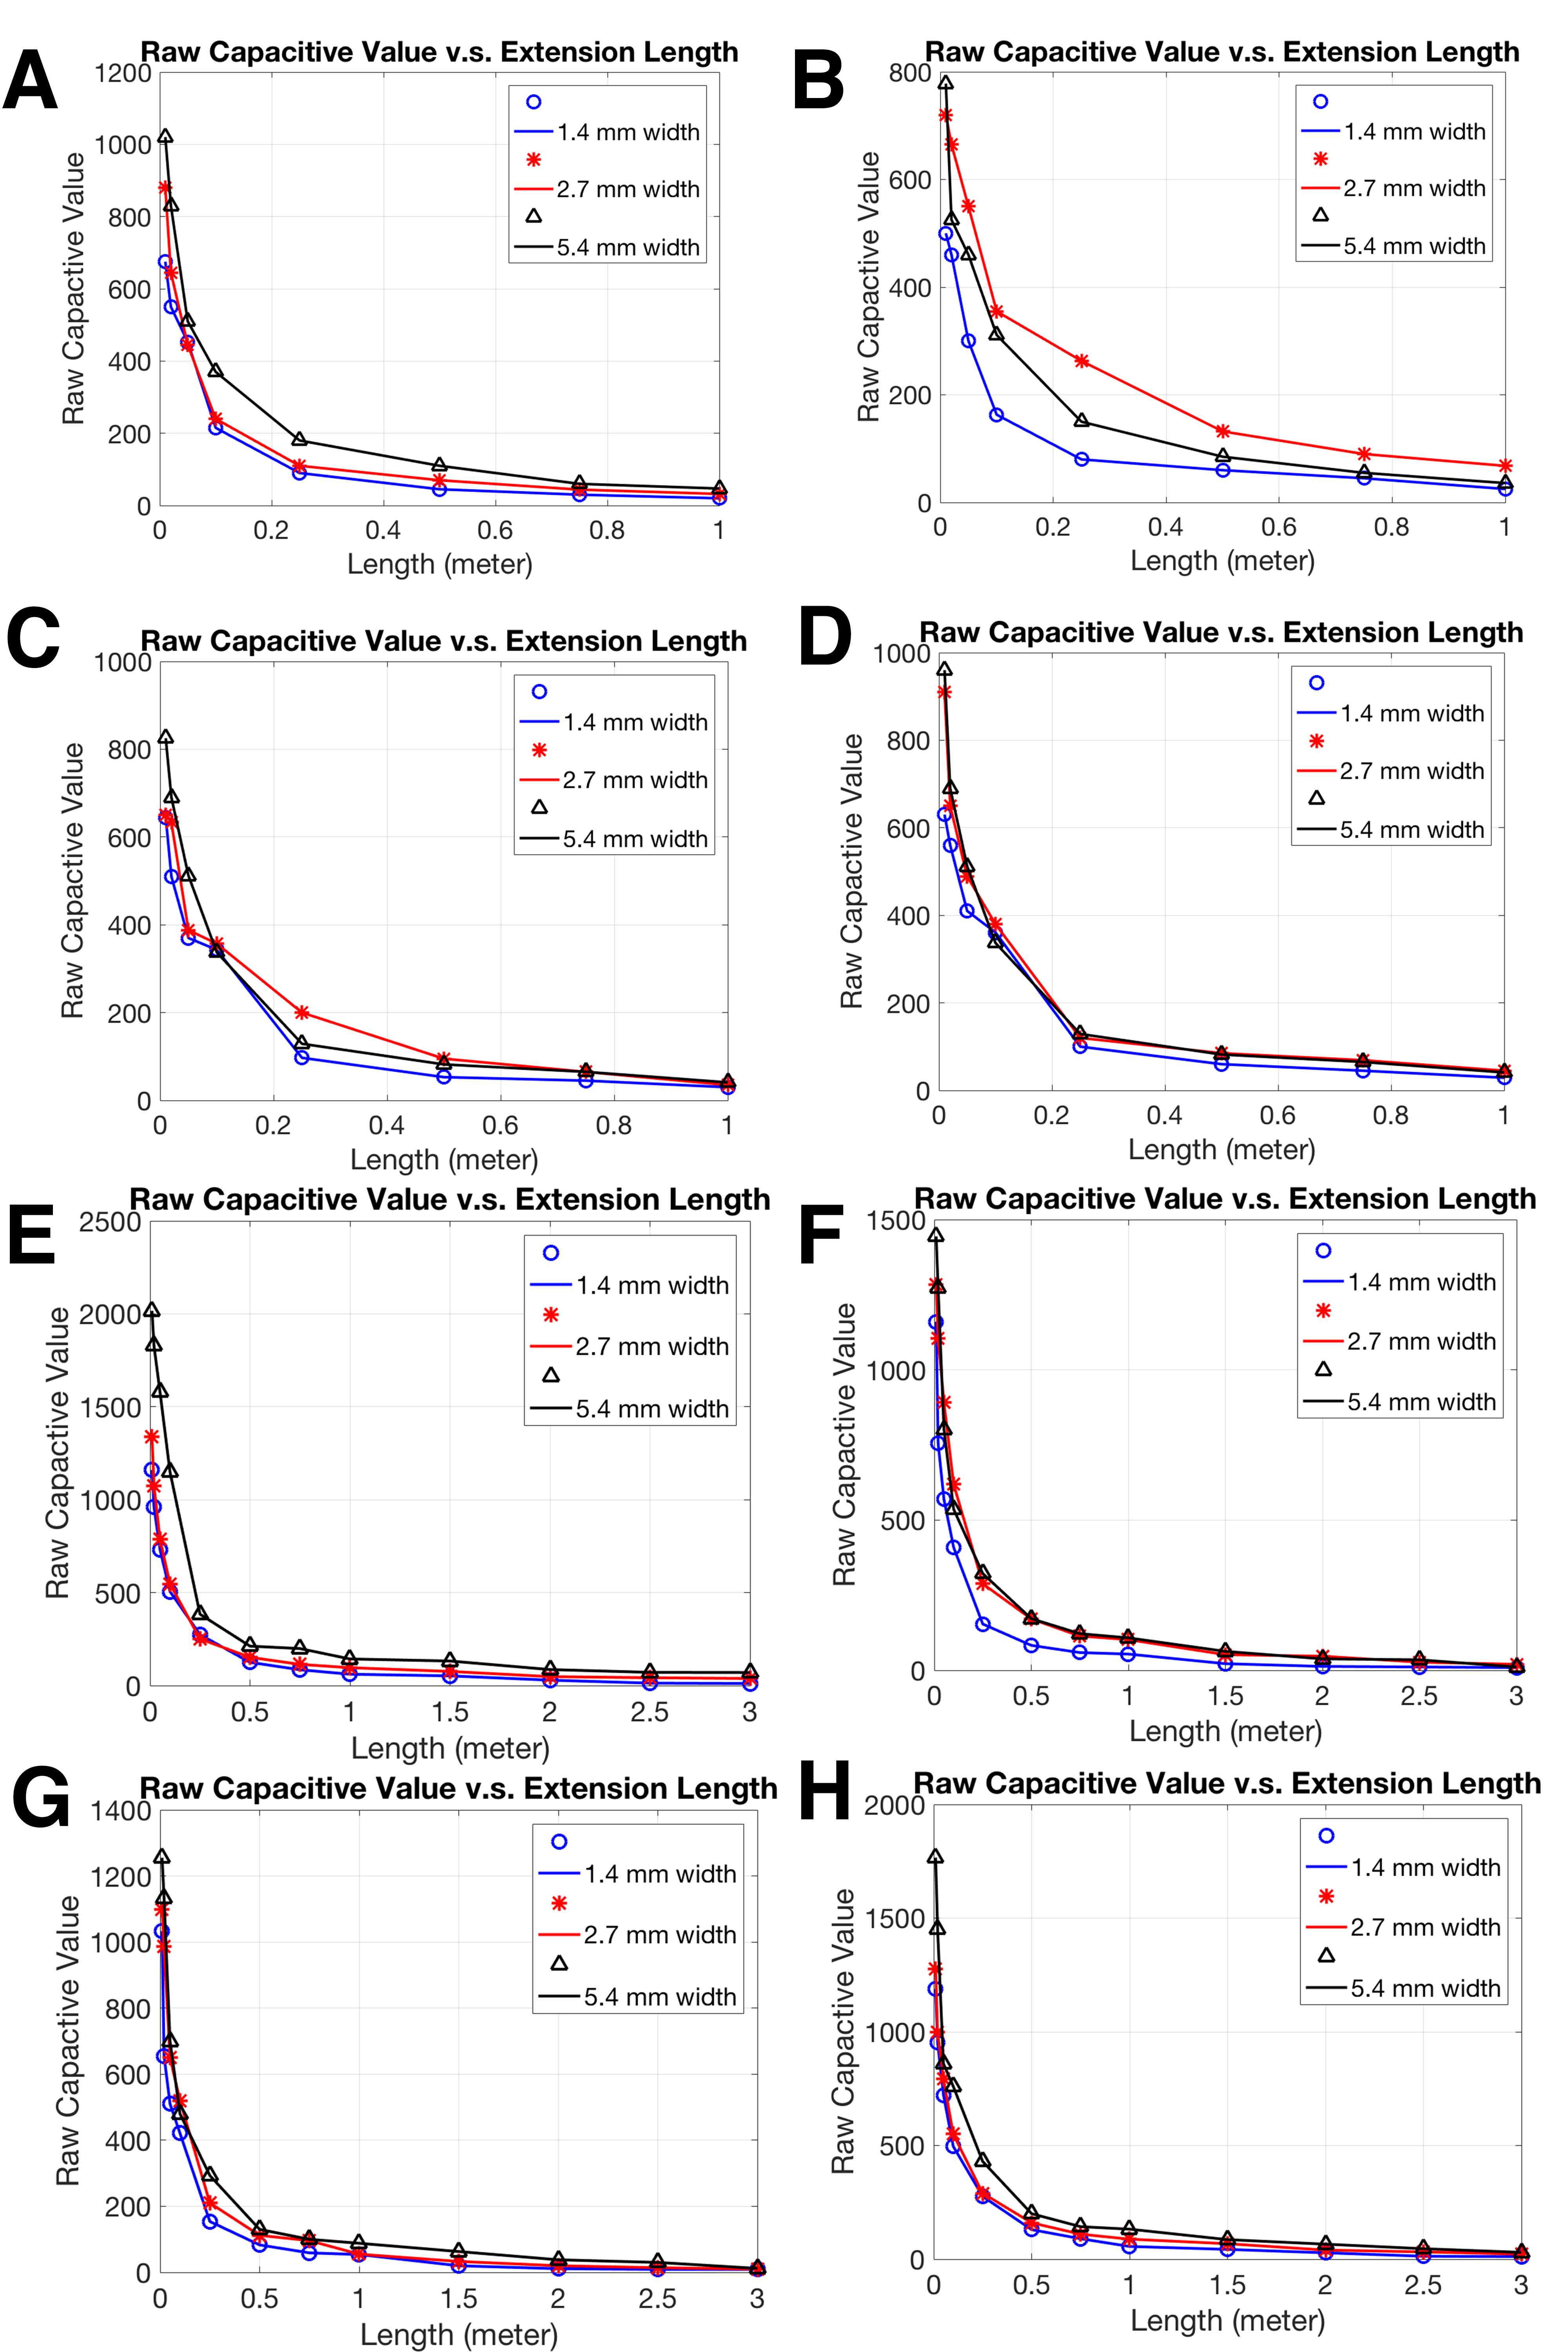
\includegraphics[width=0.65\columnwidth]{figures/length.png}
	  \caption{The curve between the increase of the raw capacitive value of the touchscreen and the lengths of the extension strip under different widths for Huawei P20 phone (A, B, C, D) and P10 phone (E, F, G, H). A/E: Copper foil tape. B/F: ITO plastic film. C/G: Carbon paint. D/H: silver nanoparticle ink.}
	  \label{fig:length}
\end{figure}


\begin{table}[ht]
\caption{Average SNR versus extension distance under different configurations. (CFT: copper foil tap, IPF: ITO PET film, CP: carbon paint, SNI: silver nanoparticle ink)}
\vspace{-2mm}
\centering
	\begin{tabular}{|c|c|c|c|c|c|c|c|c|c|c|}
	
	\hline
	\textbf{Length[m]} & \textbf{0.10} & \textbf{0.25} & \textbf{0.50} & \textbf{1.00} & \textbf{1.50} & \textbf{2.00} & \textbf{2.50} & \textbf{3.00} & \textbf{4.00} & \textbf{5.00} \\
	\hline
	P20, CFT & 6.8 & 3.5 & 1.6 & 1.1 & 0.6 & - & - & - & - & - \\\hline
    P20, IPF & 6.6 & 3.4 & 1.4 & 0.9 & 0.5 & - & - & - & - & -  \\\hline
	P20, CP &  6.5 & 3.1 & 1.9 & 0.8 & - & - & - & - & - & -  \\\hline
	P20, SNI & 6.4 & 2.9 & 1.3 & 0.9 & - & - & - & - & - & -  \\\hline
	P20, CFT w/ GND &  15.8 & 9.8 & 5.8 & 4.7 & 3.3 & 2.6 & 2.0 & 1.5 & 1.3 & 0.7 \\\hline
	P20, IPF w/ GND &  16.5 & 10.8 & 5.5 & 4.0 & 3.1 & 2.0 & 1.6 & 1.1 & 0.8 & 0.5 \\\hline
	P20, CP w/ GND & 15.4 & 10.1 & 6.0 & 3.7 & 2.2 & 1.7 & 1.0 & 0.8 & - & - \\\hline
	P20, SNI w/ GND & 15.3 & 9.8 & 5.4 & 3.1 & 2.2 & 1.7 & 1.4 & 1.2 & 0.9 & 0.5  \\\hline

	P10, CFT & 15.7 & 7.6 & 4.3 & 2.7 & 1.7 & 1.1 & 0.7 & - & - & - \\\hline
	P10, IPF  & 14.2 & 7.5 & 3.9 & 2.9 & 1.4 & 1.0 & 0.5 & - & - & - \\\hline
	P10, CP &  14.4 & 6.8 & 3.2 & 1.6 & 0.8 & 0.5 & - & - & - & - \\\hline
	P10, SNI & 14.9 & 6.9 & 3.1 & 2.8 & 1.4 & 1.0 & 0.6 & - & - & -  \\\hline
	P10, CFT w/ GND & 20.4 & 10.2 & 7.0 & 4.3 & 3.1 & 2.3 & 1.9 & 1.5 & 1.1 & 0.8 \\\hline
	P10, IPF w/ GND  &  21.4 & 11.5 & 7.9 & 5.3 & 3.2 & 2.7 & 1.7 & 1.2 & 0.8 & 0.5 \\\hline
	P10, CP w/ GND & 20.1 & 12.4 & 8.1 & 4.3 & 2.8 & 2.1 & 1.2 & 0.7 & - & - \\\hline
	P10, SNI w/ GND &  19.4 & 11.2 & 8.6 & 4.1 & 2.8 & 2.0 & 1.6 & 1.2 & 0.8 & 0.5 \\\hline
	\end{tabular}
	
	\label{tab:snrtable}
	
\end{table}

\subsection{Results}

We summarize our results in Table ~\ref{tab:snrtable}, which outlines the signal strength illustrated by the SNR value of our system. There are a total of 16 different hardware/material/grounding strip's presence configurations and each of them has ten different signal strip length configurations. We highlight the following insights gained from this evaluation study:

\textbf{1. \textit{FlexTouch} can support large-scale capacitive sensing applications with a coverage range of up to 4 meters.}  Using the  threshold of SNR > 1, we observe that the minimum sensing distance supported by \textit{FlexTouch} exceeded 0.5 meters regardless of the hardware, the material, and the grounding strip's presence. However, the grounding strip helps extend the sensing range significantly: Under the best conditions, with both the p10 and p20 hardware and CFT material, \textit{Flextouch} could reach coverage distance of more than 4 meters.

\textbf{2. \textit{FlexTouch}'s sensing range is positively correlated with material conductivity.} Among the four materials, CFT achieved the longest sensing range, following by SNI and IPF, finally by CP. This ordering is consistent with the conductivity ordering of the 4 materials presented in Figure ~\ref{fig:material-width} B. We believe that materials with even better conductivity may be able to exceed the sensing range we observed in this study. 

\begin{figure}[ht]  
\centering
  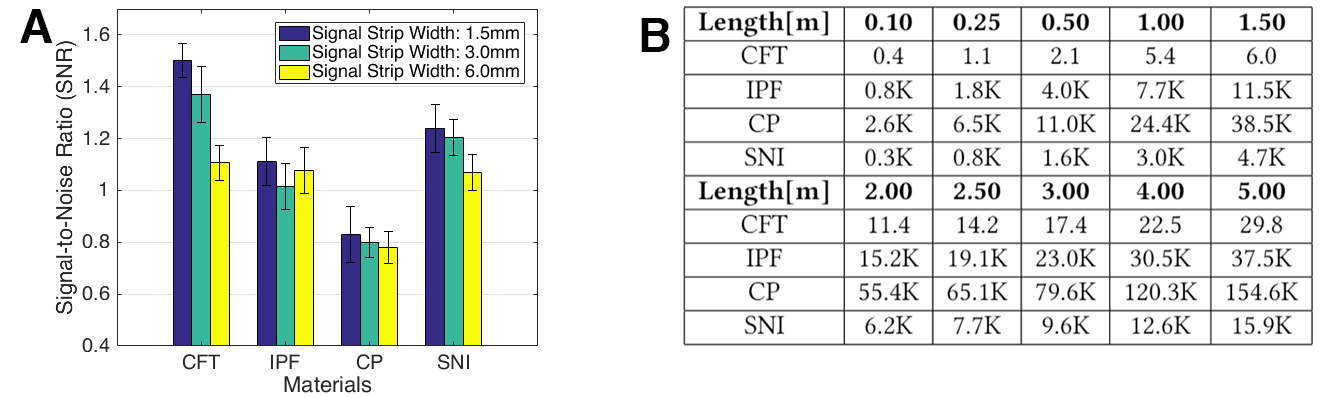
\includegraphics[width=0.95\columnwidth]{figures/material-width-and-table.png}

  \setlength{\belowcaptionskip}{-8pt}
  \caption{The SNR versus the signal strip width using four different materials (A). The table of material's resistance values ($\Omega$) under different extension lengths (B).}
  \label{fig:material-width}
\end{figure}

\textbf{3. The extension distance increases as the width of the signal strip decreases.} To better understand the effect of the width of the signal strip, we conducted a follow-up study changing the width of the signal strip made with 4 different materials with a fixed length of 3 meters. We recorded the SNR in Figure ~\ref{fig:material-width} A, which demonstrates that \textit{FlexTouch} has the best performance with a $1.5mm$-wide signal strip regardless of the fabrication material. We believe that even thinner strip will be able to support longer sensing ranges. However, since a thinner strip is less conductive, we believe that there's a lower limit on the strip's width.


\textbf{4. \textbf{\textit{FlexTouch}} can not differentiate touchpoints at different locations on the extension strip with the presence of the ground plane.} We evaluated the touch resolution on a single pair of extension strips by touching on different positions with a $50 cm$-step using different materials. We did not observe that 2D touch input could be enabled with single-layer conductive materials as prior work ~\cite{Ikematsu-Ohmic-Touch, mobicom-gao18} mentioned with the grounding strip's presence.

\textbf{5. No significant difference in using different capacitive sensing hardware}. The 2 different phones being employed in our study, Huawei p10 and P20 demonstrate moderate SNR difference when the same material is being deployed with a length below $1m$. However, when the strip length continued to increase, the SNR demonstrated similar results when all other variables are consistent. Given limited hardware resources, we were only able to evaluate these two phone models. Future studies that include capacitive touchscreens from different manufacturers will be necessary to fully understand the impact of capacitive touchscreens on the feasible sensing range of our system.

\subsection{Study Results in Relation to the Proposed Working Principle}
 
Results in Table ~\ref{tab:snrtable} show that as the length of the sensing strip increases linearly, the touch signal strength decreases logarithmically. As presented in section \textit{FlexTouch: Working Principles}, the finger touch introduces additional shunt circuit changing $C_{e}$ to $C_{eg}$. We assume the values of $C_{f}$, $C_{m}$, $C_{p}$ are 5 pF, 10 pF and 10 pF while $C_{eg} = 1.5 \times C_{e}$. Then Formula (2) can be presented as following.

Before the touch event:
\begin{equation}
    \tau_{b} = a\frac{100 + 10C_{e}}{20+C_{e}}
\end{equation}

After the finger touch on the signal strip only as well as on both the signal strip and the grounding strip: 
\begin{equation}
    \tau_{af} = a\frac{150 + 10C_{e}}{25+C_{e}}, \tau_{ag} = a\frac{150 + 15C_{e}}{25+1.5C_{e}}
\end{equation}

The estimated capacitance value can be represented as:
\begin{equation}
    \tau_{df} = \tau_{af} - \tau_{b},  \tau_{dg} = \tau_{ag} - \tau_{b}
\end{equation}

We assume that $C_{e} = 100 \times L$ where $L$ represents the length (meter) of the strip since the width is assumed to be static. The curve of how the estimated capacitive value along the strip length matches the measured raw data if $a$ is assigned to 600. The pattern we see in our result matches with the model we built for explaining \textit{FlexTouch}'s working principle. 

We measured the \textit{SNR} value by calculating the extremum of 100 data points (P20 phone, 40 data for P10 phone) without touching as the \textit{Noise} and the difference between the average of touching and non-touching as the \textit{Signal}. For instance, Figure ~\ref{fig:SNR} shows a sample of real data from the Huawei P20 phone with a 0.05m long, 2.7mm wide copper foil tape attached. Note that the noise baseline established from many measurements of parasitic capacitance is converted into digital counts. Similarly, when a finger is present, the system continues to measure the capacitance in order to establish an average value for the "touch" signal. In this case, the SNR is 18.1:1.

\begin{figure}[ht]
	\centering
	  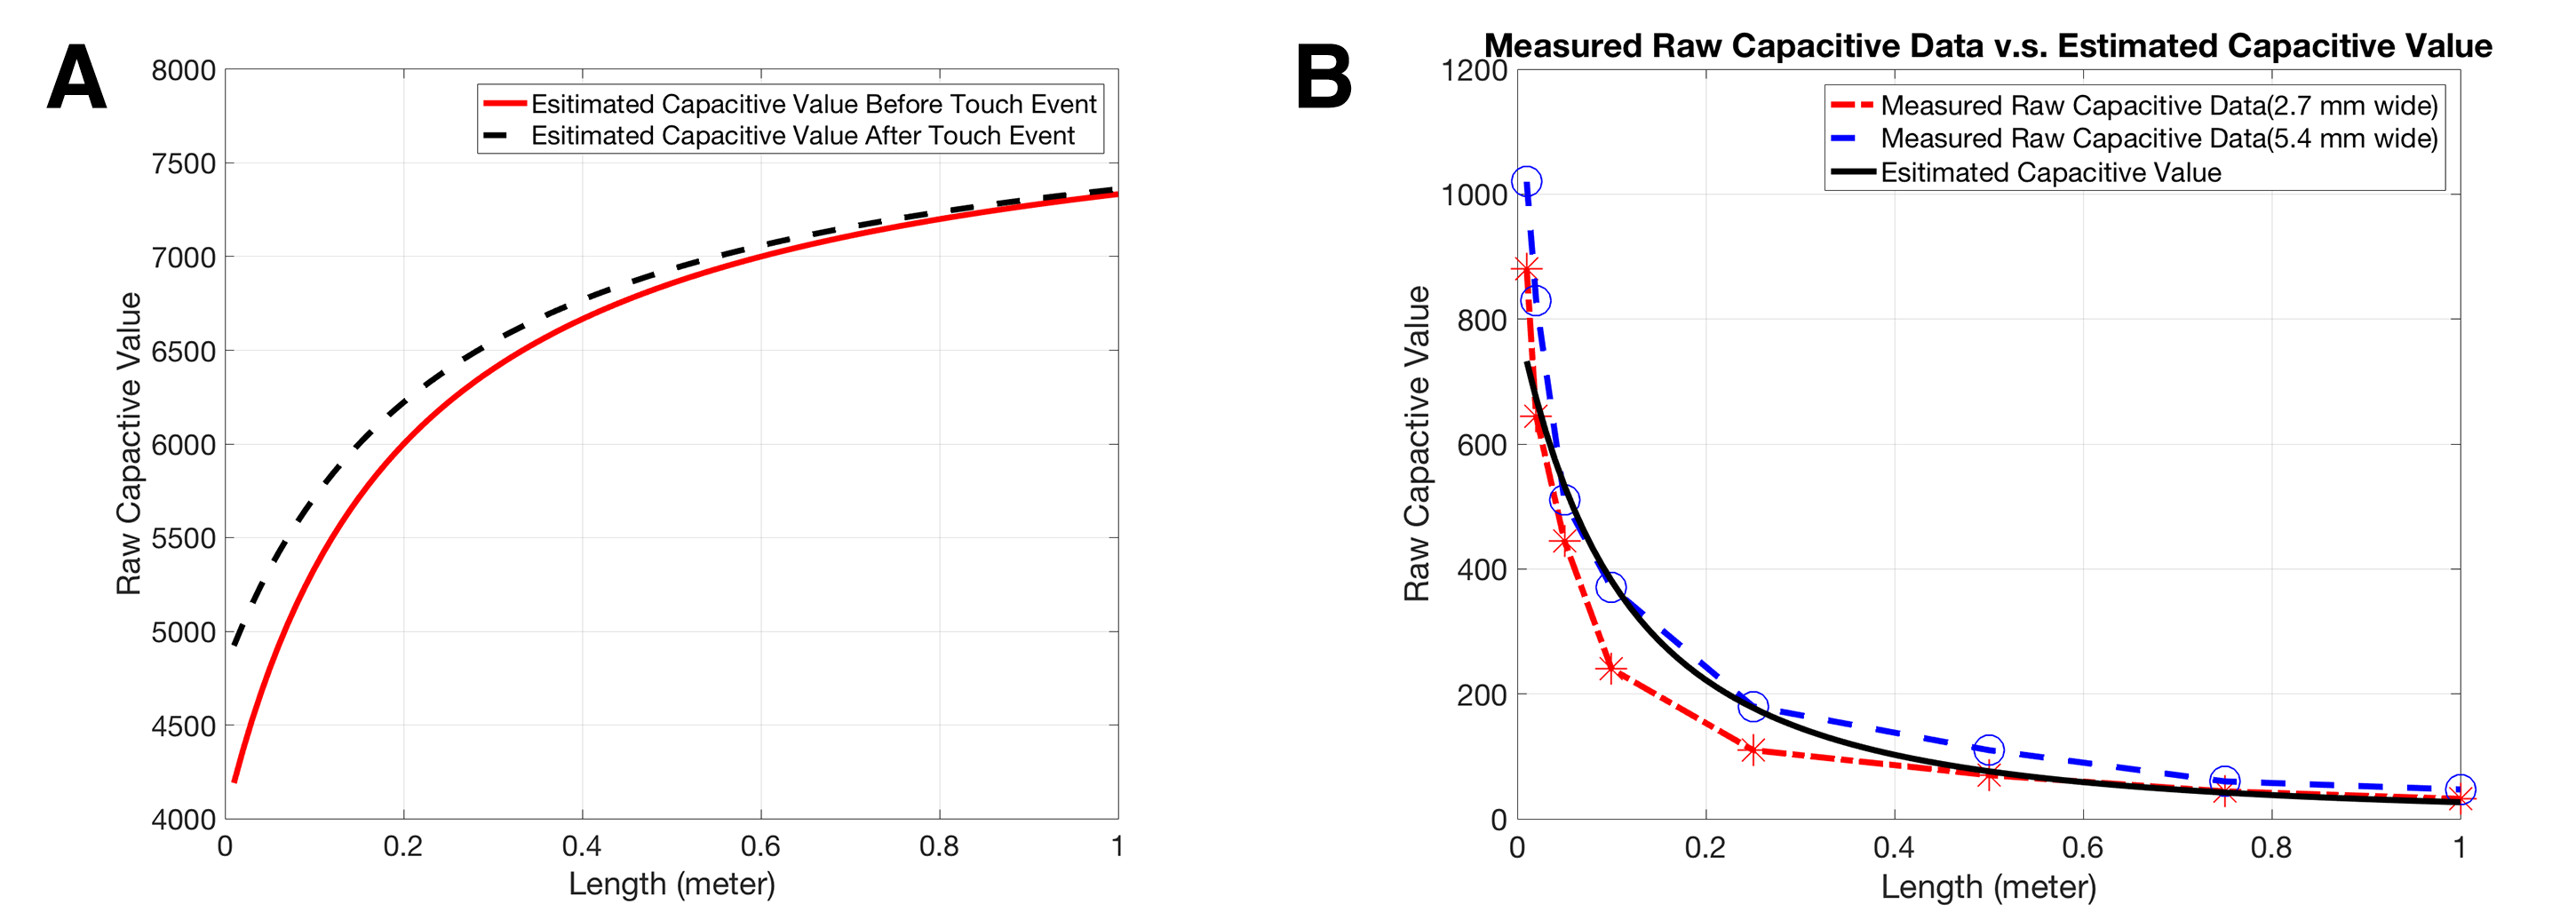
\includegraphics[width=0.95\columnwidth]{figures/estimate.png}
	  \caption{The Comparison between the measured raw capacitive data and estimated capacitive value.}
	  \label{fig:estimate}
	\end{figure}
	
	\begin{figure}
	\centering
	  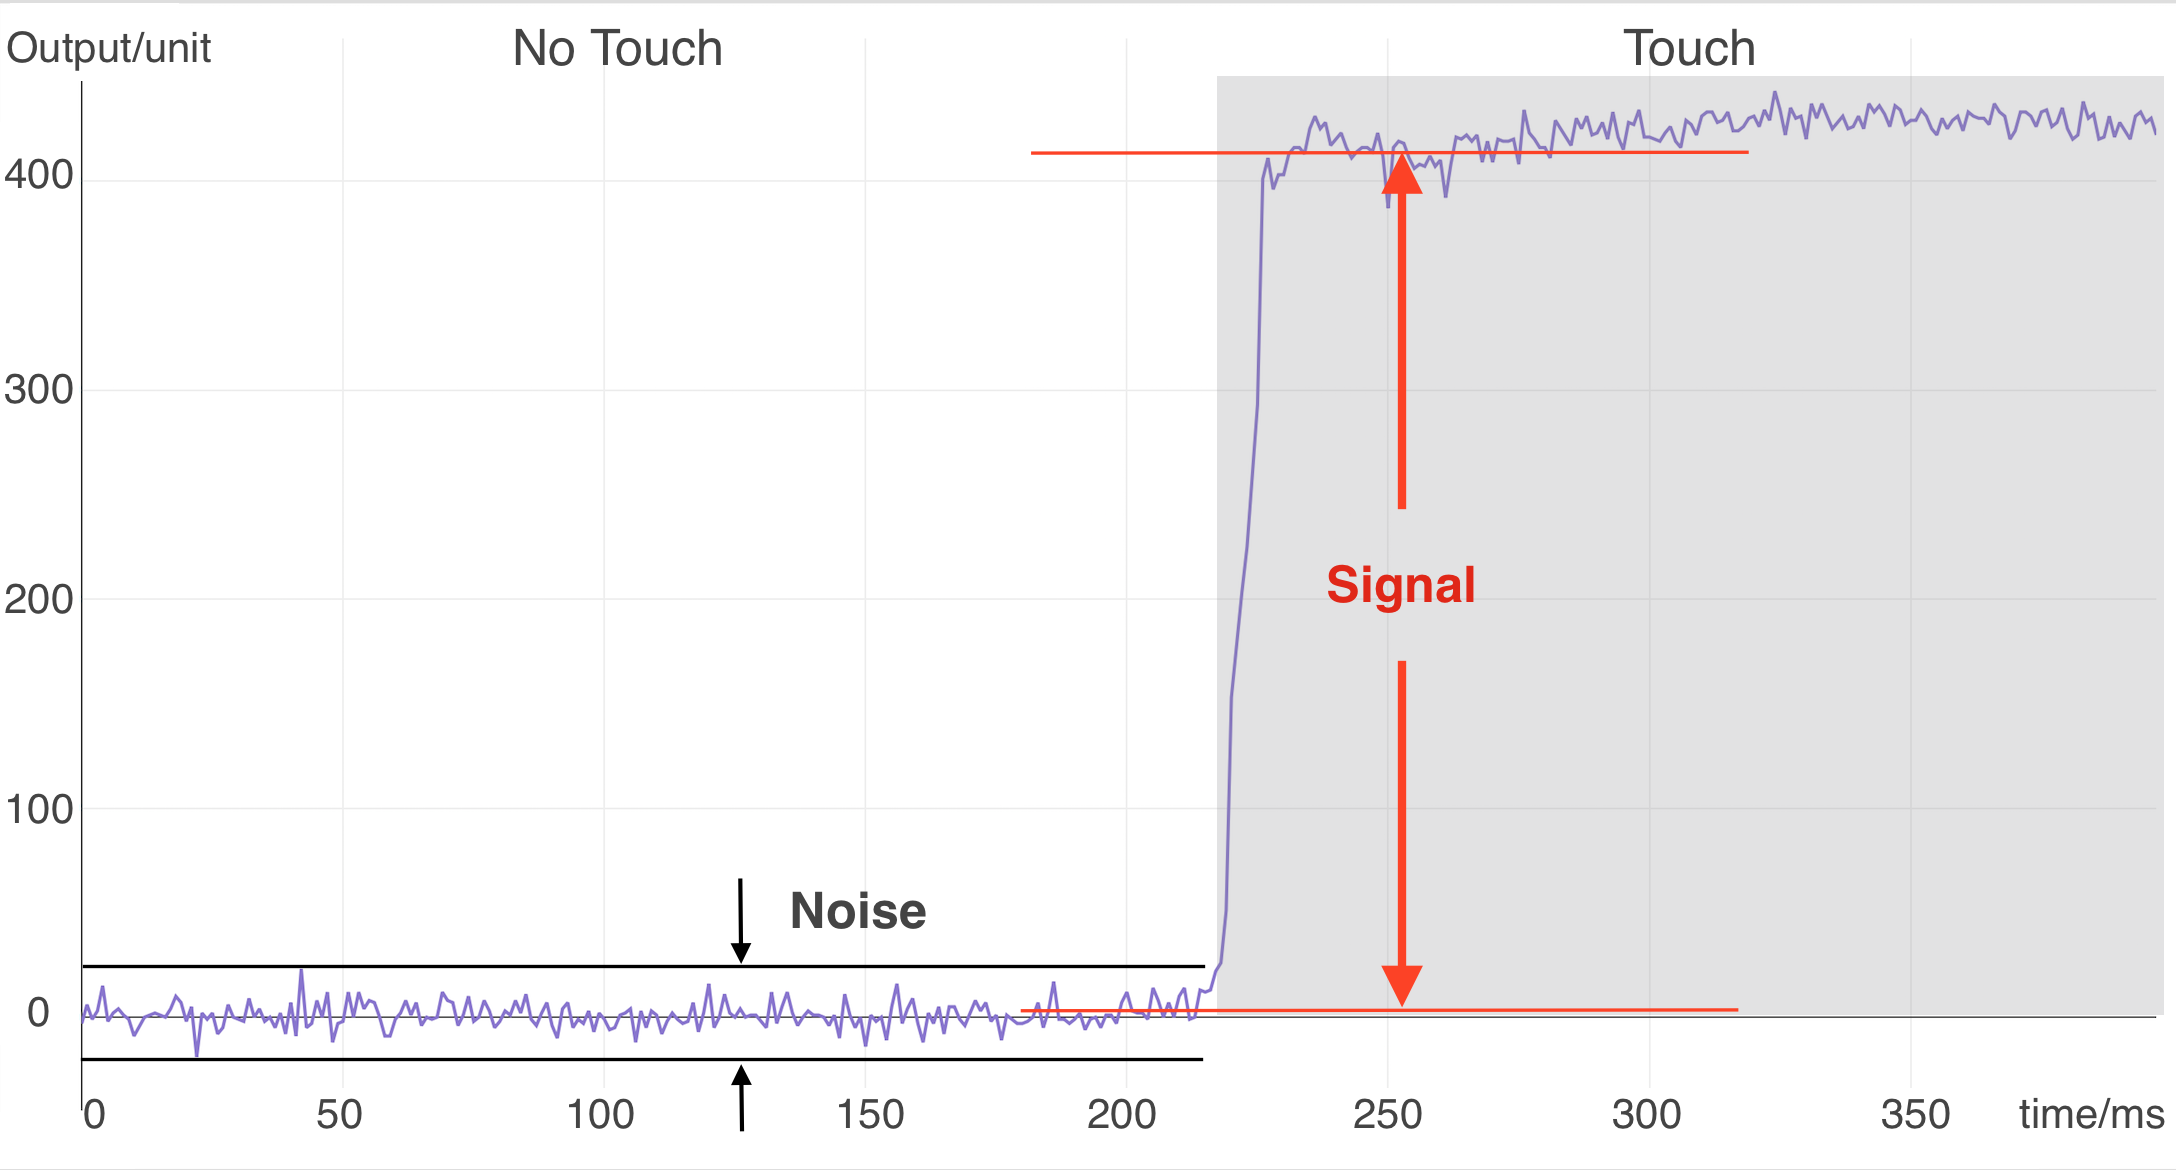
\includegraphics[width=0.95\columnwidth]{figures/SNR-definition.png}
	  \caption{The calculation of SNR with raw capacitive value from a Huawei P20 phone.}
	  \label{fig:SNR}
	\end{figure}

\section{Understanding the Effect of the Grounding Strip}
The previous study shows the significant effect of introducing the grounding strip into the extension circuit design. There are additional variables such as the distance between the grounding strip and the signal strip, the width of the grounding strip as well as the material of the grounding strip that we would like to further evaluate to provide in-depth insights into designing touch sensing solutions with \textit{FlexTouch} in this section.

\subsection{Effect of the Gap Between Grounding and Signal Strips}

We used copper foil tape as example material to examine the effect of the gap between the grounding strip and the signal strip on the maximum touch sensing distance. We set the grounding strip's width to be $6 mm$. We measured the maximum coverage with the following variables. 1) Gap distance between the central lines between the signal and grounding strips: $0.5 cm$,  $1 cm$, $2 cm$, $3 cm$, $5 cm$ and $10 cm$. 2) Signal strip's width: $1.5 mm$ and $3.0 mm$. 3) Touch postures: single index finger touch and dual index finger touch with two hands.

To measure the maximum touch sensing distance, we started with the maximum sensing distance measured in the previous study. In each session, we increased/decreased the extension distance by sticking/cutting additional $n$ pieces of $10 cm$-long copper foil tape at the far ends of both the grounding and signal strips. We recruited four participants for this study with an average age of 25.5 (SD = 1.5). They performed three touches with each touch posture at the far ends the extension strips. We repeated the above sessions until the SNR exceeded 1.0 for both single-finger and double-finger touches. We repeated the above procedure five times to obtain an average coverage distance for each condition. 

\textbf{1. The maximum touch sensing distance increases logarithmically as the gap distance between the grounding strip and signal strip increases.} As shown in Figure \ref{fig:ground-effect}, there exists an upper limit on the touching sensing coverage distance around 5 meters regarding the gap distance and the signal strip's width. However, although larger gap distance results in better sensing coverage distance, it limits the number of strips that can be deployed for any given space.

\textbf{2. Touch posture has no significant effect on the coverage distance performance.} There is no significant difference between touches with one finger or two fingers from two hands ($F_{1,89} = 0.32, p = 0.54$). We envision that future work could connect the local ground directly to users and not to the extension circuit, enabling longer sensing range and higher resolution design.


\begin{figure}[ht]
\centering
  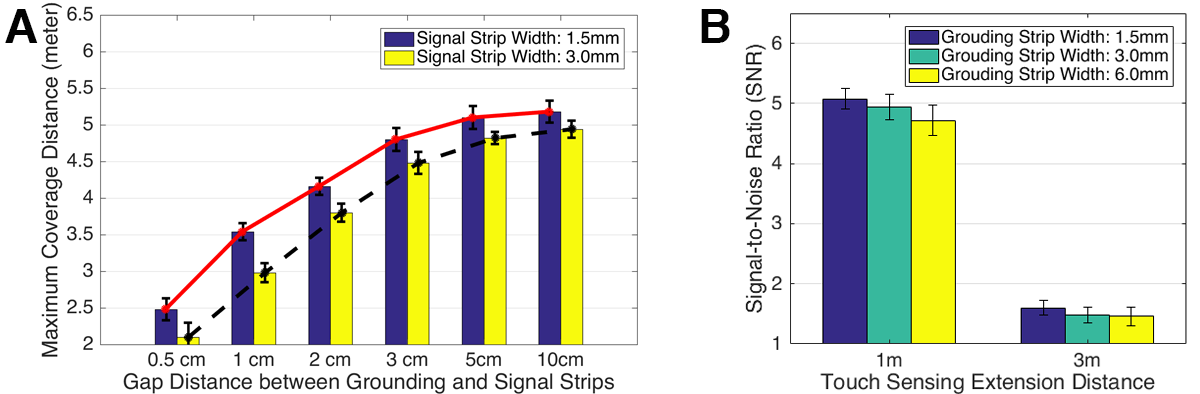
\includegraphics[width=0.95\columnwidth]{figures/grouding-gap-and-width.png}
  \setlength{\belowcaptionskip}{-8pt}
  \caption{Maximum touch sensing distance versus the gap distance between signal and grounding strips (A). SNR versus the grounding strip width with different extension distances (B).}~\label{fig:ground-effect}
\end{figure}

\subsection{Effect of Grounding Strip Width}

We used copper foil tape as example material to examine the effect of the grounding strip width on the touch sensing distance. We set the gap distance between extension strips to be $2 cm$ and the signal strip width to be $1.5 mm$. We measured the signal strength on fixed extension distances ($1m$ and $3m$) with different grounding strip's width: $1.5 mm$, $3.0 mm$ and $6 mm$. We recruited four users to touch the far ends of the paired extension strips three times for each condition. We repeated the above procedure five times to obtain an average measured SNR. We highlight the following insights gained from this evaluation study:


\textbf{The touch sensing coverage distance is negatively correlated with the grounding strip's width.} We recorded the SNR values in Figure \ref{fig:ground-effect} B, which demonstrates that \textit{FlexTouch} has the best performance with the $1.5mm$-wide signal strip. We recommend a thinner signal strip that can support better sensing range performance as well as higher resolution design. Combined with the result on the signal strip's width in Section $5.1.1$, we believe that the sensing distance can be further extended if we adopt $1.5 mm$-wide or thinner copper foil tape for both the signal and grounding strips.

\subsection{Effect of the Grounding Strip Material}
In this study, we explored whether grounding strip material affects the sensing distance performance. We set the signal strip material to be copper foil tape, the gap distance between extension strips to be $2 cm$ and the widths of both the signal strip and grounding strip to be $6.0 mm$. We measured the SNR values of 1-meter and 3-meters sensing distance with four different grounding strip's materials. The result is illustrated in Table \ref{tab:gnd-material}.

\begin{table}[ht]
\caption{Average (standard deviation) SNR values with one strip made of CFT and the other made of one of the three materials.}
\vspace{-2mm}
\resizebox{\textwidth}{12mm}{
\centering
	\begin{tabular}{|c|c|c|c|c|c|c|c|}
	\hline
	Material &\textbf{CFT} & \multicolumn{2}{c|}{\textbf{IPF}} & \multicolumn{2}{c|}{\textbf{CP}} & \multicolumn{2}{c|}{\textbf{SNI}} \\
	\hline
    Condition & \textbf{reference} & \textbf{ground} & \textbf{signal} & \textbf{ground} & \textbf{signal} & \textbf{ground} & \textbf{signal}  \\
	\hline
	
	$1m$ sensing distance & 1.14 (0.07) & 1.06 (0.11) & 1.07 (0.13) & 0.88 (0.12) & 0.86 (0.10) & 1.11 (0.14) & 1.09 (0.13) \\
	\hline
	$3m$ sensing distance & 3.40 (0.20) & 3.31 (0.25) & 3.35 (0.23) & 3.22 (0.12) & 3.20 (0.08) & 3.42 (0.13) & 3.37 (0.14)   \\
	\hline
	\end{tabular}}
	\label{tab:gnd-material}
	
\end{table}

\textbf{1. \textit{FlexTouch} sensing range is positively correlated with material conductivity of the \textit{grounding strip} in general.} Similar to the results in Section \textit{5.1.1}, we found that the material conductivity has a positive effect on the sensing range performance.

Then we switched the grounding strip and the signal strip which are made of different materials and noticed that:
 
\textbf{2. Signal strip and ground strip made of different materials are interchangeable when they have the same width.} We found no significant difference in the signal strength when switched the two strips with the same width but different materials. 

\subsection{Study Results in Relation to the Proposed Working Principle }
Section $5.1.2$ explains the relationship between signal strength and the extension strip's length using the working principle hypotheses in Section $3$. We explain the results we found in study 2 that pertain to the effect of separation - $d$ as well as fabrication material - $\varepsilon$.

To enhance the effect introduced by touch, less capacitance between the signal strip and the grounding strip is preferred, which is represented as $C_{e}$. The sensing distance can be represented as: 

\begin{equation}
    L = \frac{C_{e} \times d}{\varepsilon \times D}
\end{equation}

Therefore, we conclude that smaller extension strip width ($D$), larger gap distance ($d$), more conductive material and more insulating material between strips (smaller $\varepsilon$) will help extend the sensing range, which is consistent with our study's results.

\section{Evaluating Object Presence Sensing Capabilities}
Given the capacitive nature of \textit{FlexTouch}'s sensing principle, it can go beyond sensing touch events. Everyday objects that contain capacitance also draw electric current from the touchscreen and can be detected by \textit{FlexTouch}. In this section, we evaluate the feasibility of detecting everyday objects' presence using \textit{FlexTouch}. 

\subsection{Apparatus and Procedure}
In this study, we used $3.0 mm$ wide copper foil tape and a Huawei P20 phone. We explored a range of factors that may affect \textit{FlexTouch}'s capability in sensing everyday objects' presence: the dielectric property and materials of different everyday objects, the length of the extension strips as well as the presence of the local ground. We used the following procedure in the experiment:

1) We attached the signal strip to the central position of the 19th sensing node on the left edge of the touchscreen. Then we started the testing application on the phone sending the raw capacitive data to a local server running on a laptop for later analysis.

2) We placed 11 pre-selected objects in random order at the end of the signal strip without the grounding strip's presence for around 2 seconds then on both the signal and grounding strips for another 2 seconds. We picked up and re-placed the object five times, ensuring the object was in contact with the strips on each placement.

3) We trimmed the strips in order of the following lengths: 3m, 2m, 1.5m, 1m, 0.5m, 0.25m, 0.1m and repeated step 2).

\subsection{Results}

Table ~\ref{tab:snrtableforobj} presents the average SNR value with 22 configurations across everyday objects and the presence of the grounding strip.

As presented in Table ~\ref{tab:snrtableforobj}, \textit{FlexTouch} can sense the presence of everyday objects by detecting the current they draw via the extension strip. The second column in Table ~\ref{tab:snrtableforobj} illustrates that all the objects change the capacitive signal extended from the touchscreen on the phone. However, the sensing range varies with the object's material. Objects made of metal have the strongest signal strength. The coverage distance ranges from $50 cm$ to $2 m$. Besides, pairing the local ground with the touch screen extension strip can dramatically enhance the object detection's sensing range. 


\begin{table}[ht]
\caption{Average SNRs versus extension strips' lengths with different everyday objects. The table's X and  Y values (X/Y) represents the SNR values of conditions with and without the grounding strip. }
\vspace{-2mm}
	\centering
		\begin{tabular}{|c|c|c|c|c|c|c|c|c|}
		\hline
		\textbf{Length[m]} & \textbf{0.10} & \textbf{0.25} & \textbf{0.50} & \textbf{1.00} & \textbf{1.50} & \textbf{2.00} & \textbf{3.00} \\
		\hline
		Finger Touch (\textbf{reference}) & 15.8/6.8 & 9.8/3.5 & 5.8/1.6 & 4.7/1.1 & 3.3/0.6 & 2.6/- & 1.5/-  \\\hline
		$5 cm\times 5 cm$ Copper Foil Tape & 15.3/3.2 & 9.5/1.9 & 5.5/0.8 & 4.6/- & 3.0/- & 2.3/- & 1.3/-  \\\hline
		Stainless Steel Water Cup &  12.6/3.4 & 10.0/2.0 & 4.3/1.1 & 2.0/- & 1.6/- & 1.5/- & 0.7/-  \\\hline
		MacBook Pro 13' &  5.4/2.4 & 3.7/1.7 & 1.2/0.6 & 0.6/- & -/- & -/- & -/- \\\hline
		Carving Knife  & 5.6/1.5 & 2.7/0.6 & 1.3/- & -/- & -/- & -/- & -/-  \\\hline
		iPhone XR  & 4.6/2.5 & 2.5/2.0 & 1.2/0.5 & 0.7/- & -/- & -/- & -/- \\\hline
		550 ml Bottled Water  &  4.3/2.8 & 2.8/1.2 & 0.6/- & -/- & -/- & -/- & -/- \\\hline
		50 ml Bottled Water  &  3.1/1.3 & 2.0/0.7 &  -/- & -/- & -/- & -/- & -/- \\\hline
		Glass Cup &  2.7/0.6 & 1.0/- & -/- & -/- & -/- & -/- & -/-  \\\hline
		Notebook & 0.9/0.8 & -/- & -/- & -/- & -/- & -/- & -/-   \\\hline
		Cardboard Box  & 0.5/0.6 & -/- & -/- & -/- & -/- & -/- & -/-  \\\hline
		Mouse & 0.5/0.5 & -/- & -/- & -/- & -/- & -/- & -/- \\\hline
		\end{tabular}
		
		\label{tab:snrtableforobj}
		
\end{table}



